\chapter{Mediciones y resultados}
En este capítulo se presentan los resultados del diseño del protocolo SPI utilizado para controlar los convertidores D/A y A/D, así como los resultados obtenidos de la caracterización de resistencias, multiplexores y fotorresistencia. Además, se muestran las imágenes generadas por la matriz de fototransistores, evidenciando el correcto funcionamiento del sistema de adquisición de datos implementado y de la PCB diseñada.


\section{Resultados de protocolo SPI}
Para probar el funcionamiento del diseño del protocolo SPI, se utilizó un potenciómetro al que se varió la resistencia, conectado a un canal del convertidor A/D. Para evaluar el convertidor D/A, se asignó un valor de voltaje en formato binario. Las señales generadas por los módulos implementados en la FPGA, junto con las conversiones realizadas por el ADC y DAC, fueron visualizadas mediante un osciloscopio y un multímetro. En esta sección se explicarán los resultados obtenidos de ambos convertidores.

\subsection{ADC}
En el ADC se utilizó el protocolo de lectura y escritura del SPI. De acuerdo al datasheet, una conversión completa requiere 25 ciclos de dclk: durante los primeros 8 ciclos se configura el ADC, luego se deja pasar un ciclo, y en los siguientes 16 ciclos se realiza la conversión. El ADC realiza la conversión en grupos de 8 bits.


En las capturas del osciloscopio (Figura \ref{fig:ss_osc_adc_2v} y Figura \ref{fig:ss_osc_adc_3v}) se visualizan cuatro señales numeradas del 1 al 4. La señal 1 corresponde al comando de configuración del ADC, la señal 2 al reloj dclk, la señal 3 a la conversión realizada por el ADC, y la señal 4 al chip select (CS). Es importante destacar que las señales 1, 2, y 4 son generadas por los módulos diseñados e implementados en la FPGA, mientras que la señal 3 proviene directamente del ADC, mostrando el resultado de la conversión.


Se realizaron dos pruebas para comprobar el funcionamiento del SPI. En la primera se conectó un potenciómetro al canal 0 del ADC y se configuró hasta obtener un voltaje de 2V. En la Figura \ref{fig:ss_osc_adc_2v} se muestra la conversión realizada por el dispositivo, evidenciando el funcionamiento del diseño del protocolo SPI y del ADC al realizar la conversión de la señal analógica a digital.

            \begin{figure}[hbtp]
                \centering
                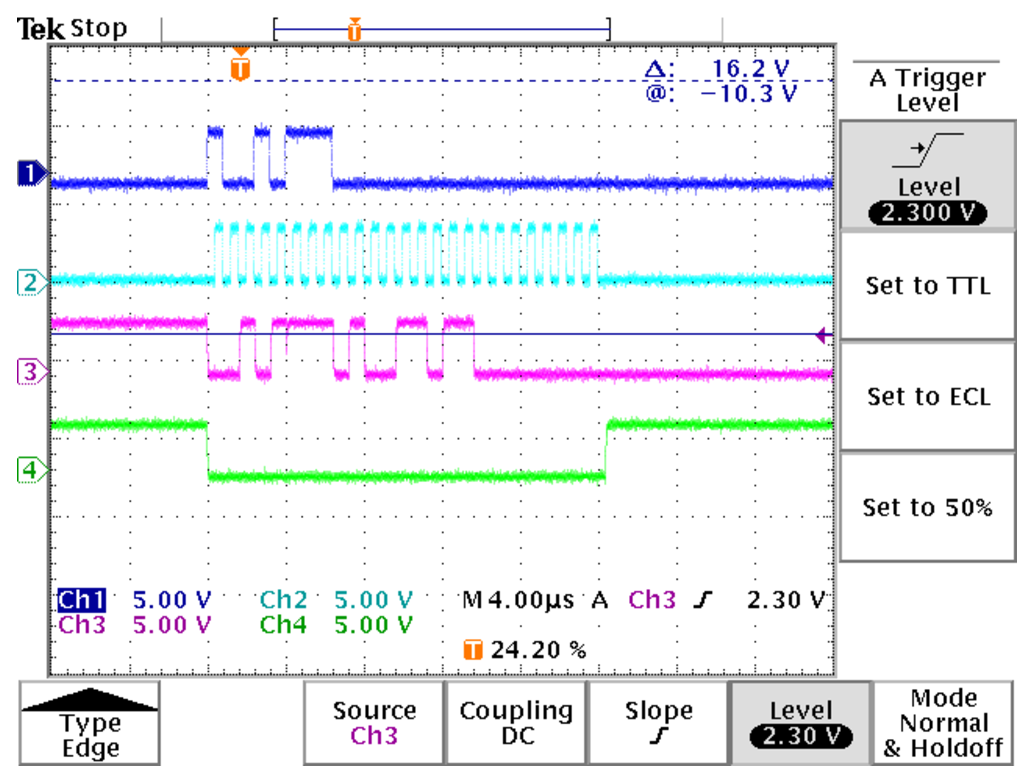
\includegraphics[width=0.6\textwidth]{ss_osc_adc_2v}
                \caption{Captura de osciloscopio de la conversión de 2V realizada por el ADC.}
                \label{fig:ss_osc_adc_2v}
            \end{figure} 

La conversión en el ADC comienza a partir del décimo pulso del dclk. En este caso, la conversión resultante fue 1001 1011 0000, lo que equivale a 2480 en decimal. Realizando una regla de tres, se obtiene que este valor corresponde a un voltaje de 1.9985V.


La segunda prueba consistió en aplicar 3.3V al canal 0 del ADC para evaluar su respuesta ante un voltaje mayor. En la siguiente figura se muestra la conversión resultante
            \begin{figure}[hbtp]
                \centering
                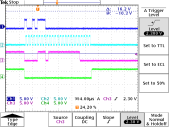
\includegraphics[width=0.6\textwidth]{ss_osc_adc_3v}
                \caption{Captura de osciloscopio de la conversión de 3.3V realizada por el ADC.}
                \label{fig:ss_osc_adc_3v}
            \end{figure} 

El resultado de la conversión fue 1111 1111 1111, que corresponde a 4095 en decimal. Este valor equivale a un voltaje de 3.3V, confirmando que el ADC realizó correctamente la conversión de la señal analógica al valor digital máximo posible para este canal.
     
\subsection{DAC}
Para controlar el DAC, se utilizó únicamente la escritura a través del protocolo SPI. Basándonos en el datasheet del DAC, la escritura se realiza en 16 ciclos de sck. Durante los primeros 4 ciclos, se envía el comando de configuración, en el cual se especifica en qué canal se tendrá el resultado de la conversión. En los 12 ciclos restantes, se transmite un valor de voltaje en formato binario de 12 bits al dispositivo para su conversión a señal analógica.


En las Figuras \ref{fig:ss_osc_dac_2v} y \ref{fig:ss_osc_dac_3v} se muestran las capturas del osciloscopio, donde se pueden observar tres señales numeradas del 1 al 3. La señal número 1 corresponde a los pulsos de reloj sck, la señal número 2 muestra el comando y el valor del voltaje en formato binario, y la señal número 3 representa el chip select del dispositivo. Todas estas señales fueron generadas por los módulos de diseño del protocolo SPI implementado.


Para verificar que el DAC realizara correctamente la conversión, se asignaron dos valores de voltaje en formato binario al MOSI: 1001 1011 0010, equivalente a 2V, y 1111 1111 1111, equivalente a 3.3V. Posteriormente, se midió el voltaje en el canal asignado utilizando un multímetro, confirmando que las conversiones fueron precisas.


En las siguientes imágenes se muestran las capturas del osciloscopio correspondientes a la escritura del DAC, así como el resultado de la conversión de 2V y 3.3V, respectivamente.

            \begin{figure}[hbtp]
                \centering
                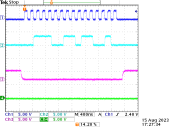
\includegraphics[width=0.6\textwidth]{ss_osc_dac_2v}
                \caption{Captura de osciloscopio de la escritura de 2V en binario en el DAC.}
                \label{fig:ss_osc_dac_2v}
            \end{figure}
            
            \begin{figure}[hbtp]
                \centering
                \includegraphics[width=0.6\textwidth]{dac_conversion_2v}
                \caption{Resultado de la conversión de 2V realizada por el DAC.}
                \label{fig:dac_conversion_2v}
            \end{figure}            
          
            \begin{figure}[hbtp]
                \centering
                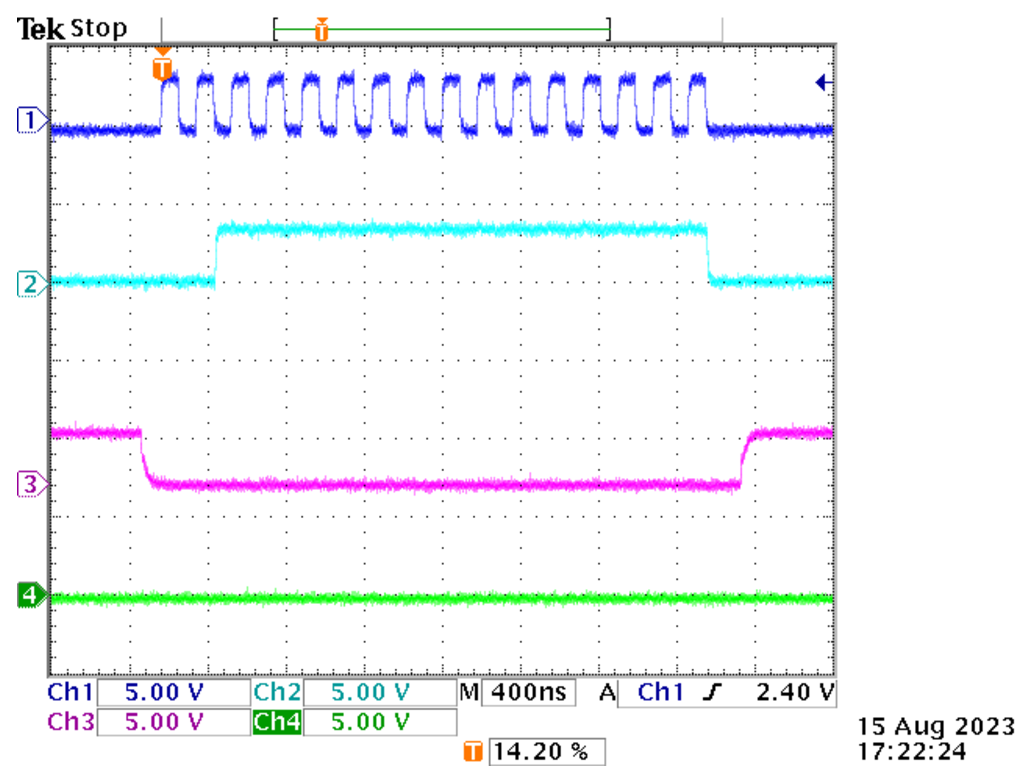
\includegraphics[width=0.6\textwidth]{ss_osc_dac_3v}
                \caption{Captura de osciloscopio de la escritura de 3.3V en binario en el DAC}
                \label{fig:ss_osc_dac_3v}
            \end{figure}   

            \begin{figure}[hbtp]
                \centering
                \includegraphics[width=0.6\textwidth]{dac_conversion_3v}
                \caption{Resultado de la conversión de 3.3V realizada por el DAC.}
                \label{fig:dac_conversion_3v}
            \end{figure} 
                                 
\section{Resultados de caracterización de resistencias}  
Al trabajar con la matriz de resistencias y al integrar los multiplexores en el sistema, se observó que el valor de voltaje recibido era menor de lo esperado. Este comportamiento anómalo llevó a sospechar que los multiplexores estaban introduciendo una resistencia adicional que afectaba las mediciones. Para investigar el impacto de esta resistencia en los resultados, se optó por medir la resistencia interna de los multiplexores. Esta medición permitió cuantificar el efecto de los multiplexores sobre los valores de voltaje obtenidos y ajustar el diseño para minimizar el impacto de esta resistencia en las lecturas.
            \begin{table}[htbp]
                \caption{Resistencia de multiplexores.}
                \begin{center}
                    \resizebox{0.9\linewidth}{!}{ 
                    \begin{NiceTabular}{| c | c | c | c | c | c |}
                        \CodeBefore
                        \Body
                        \hline
                        \textbf{$R_{test}$}  & \textbf{$V_{muxrows}$} & \textbf{$V_{muxcols}$} & \textbf{$i$} & \textbf{$R_{mux_{row}}$} & \textbf{$R_{mux_{col}}$}\\
                        \hline
                        1K$\Omega$   & 3.86e-2 V& 3.5e-2  V& 2.65e-4 A& 145.66 $\Omega$& 132$\Omega$\\
                        3.3K$\Omega$ & 3.43e-2 V& 3.1e-2  V& 2.21e-4 A& 155.2 $\Omega$& 140.27$\Omega$\\
                        5.6K$\Omega$ & 2.83e-2 V& 2.48e-2 V& 1.89e-4 A& 149.73 $\Omega$& 131.21$\Omega$\\
                        10K$\Omega$  & 2.25e-2 V& 2.11e-2 V& 1.49e-4 A& 151 $\Omega$& 141.6$\Omega$\\                            
                        \hline
                    \end{NiceTabular}
                    }
                \label{tab:Mux_res}
                \end{center}
            \end{table}

            \begin{figure}[hbtp]
                \centering
                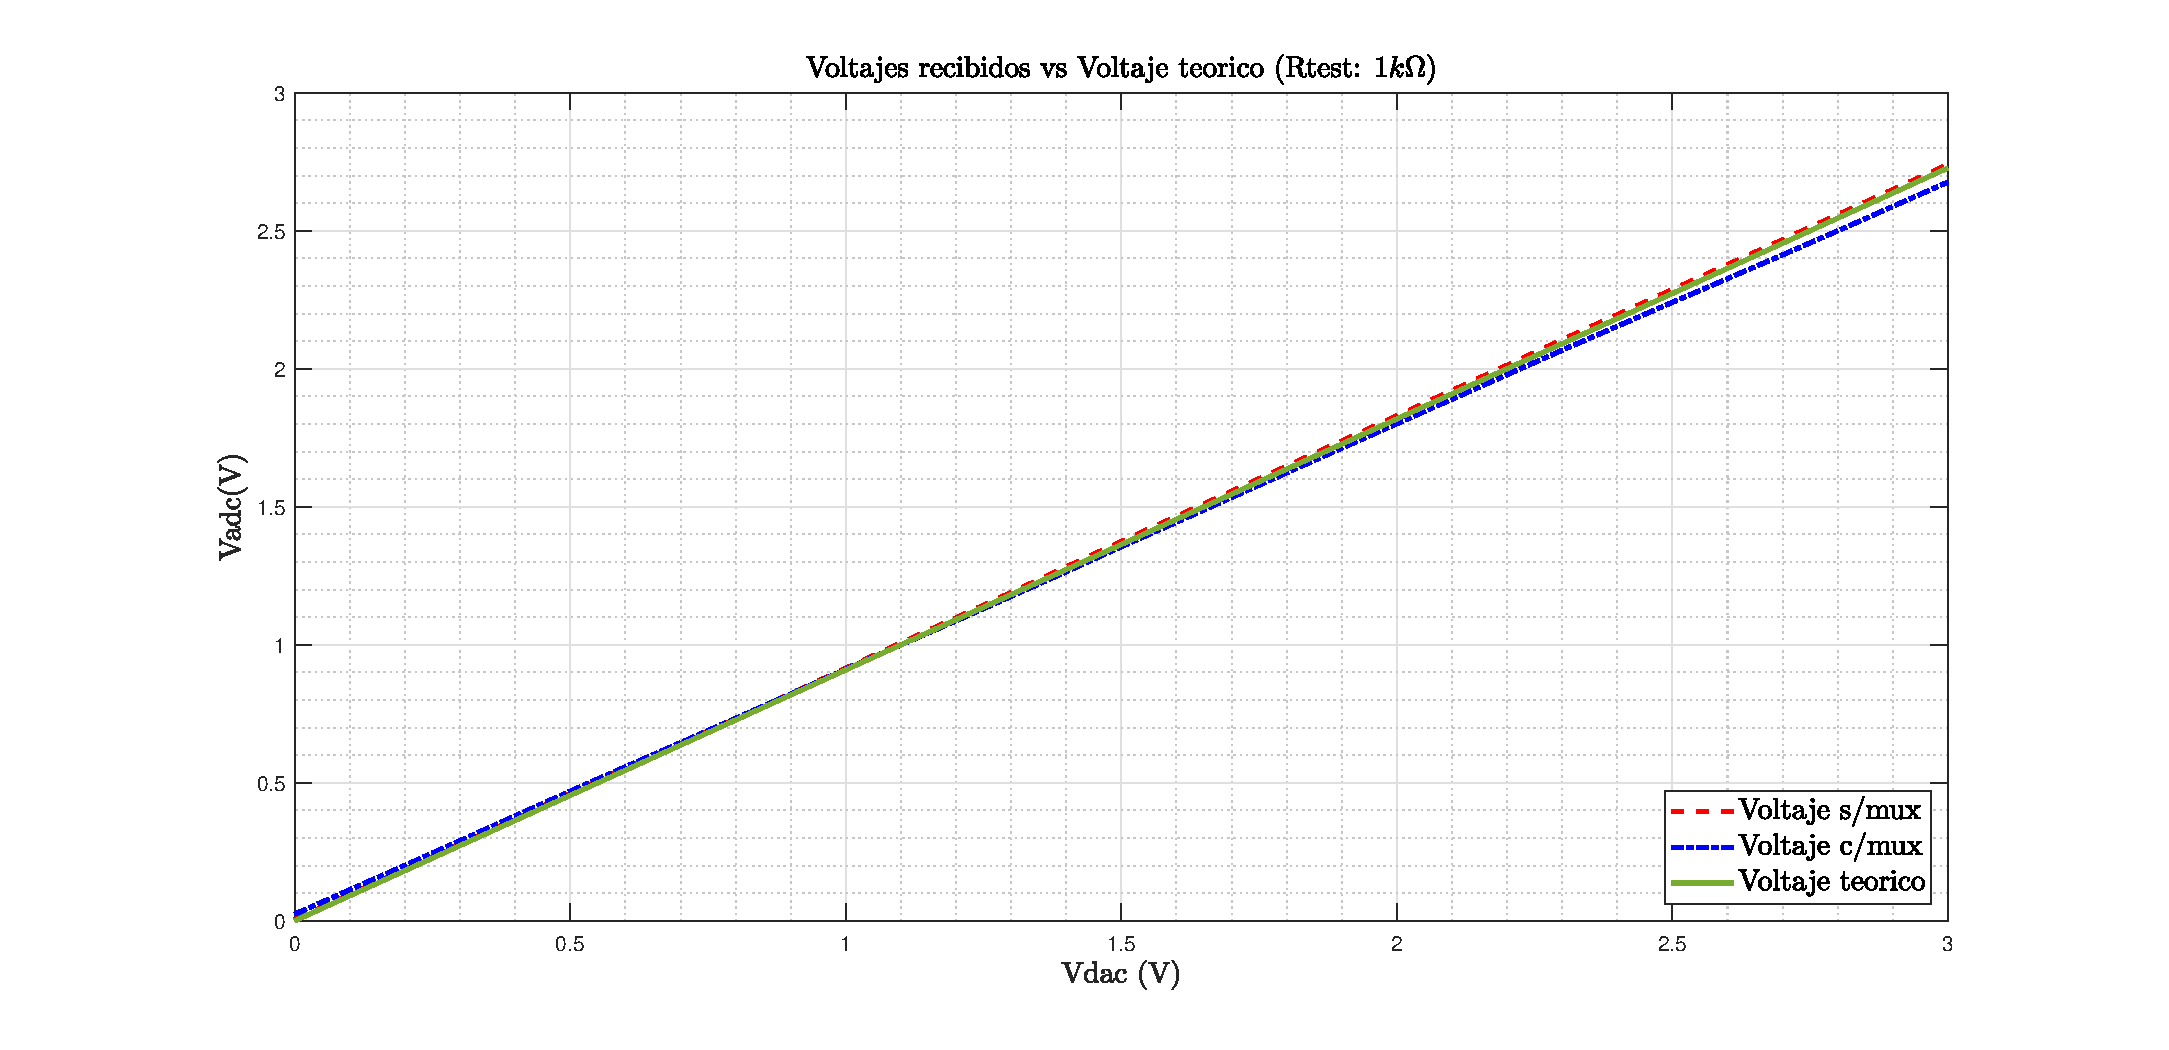
\includegraphics[width=1\textwidth]{01_1k}
                \caption{Influencia de resistencia de multiplexores.}
                \label{fig:01_1k}
            \end{figure}  
            
            \begin{figure}[hbtp]
                \centering
                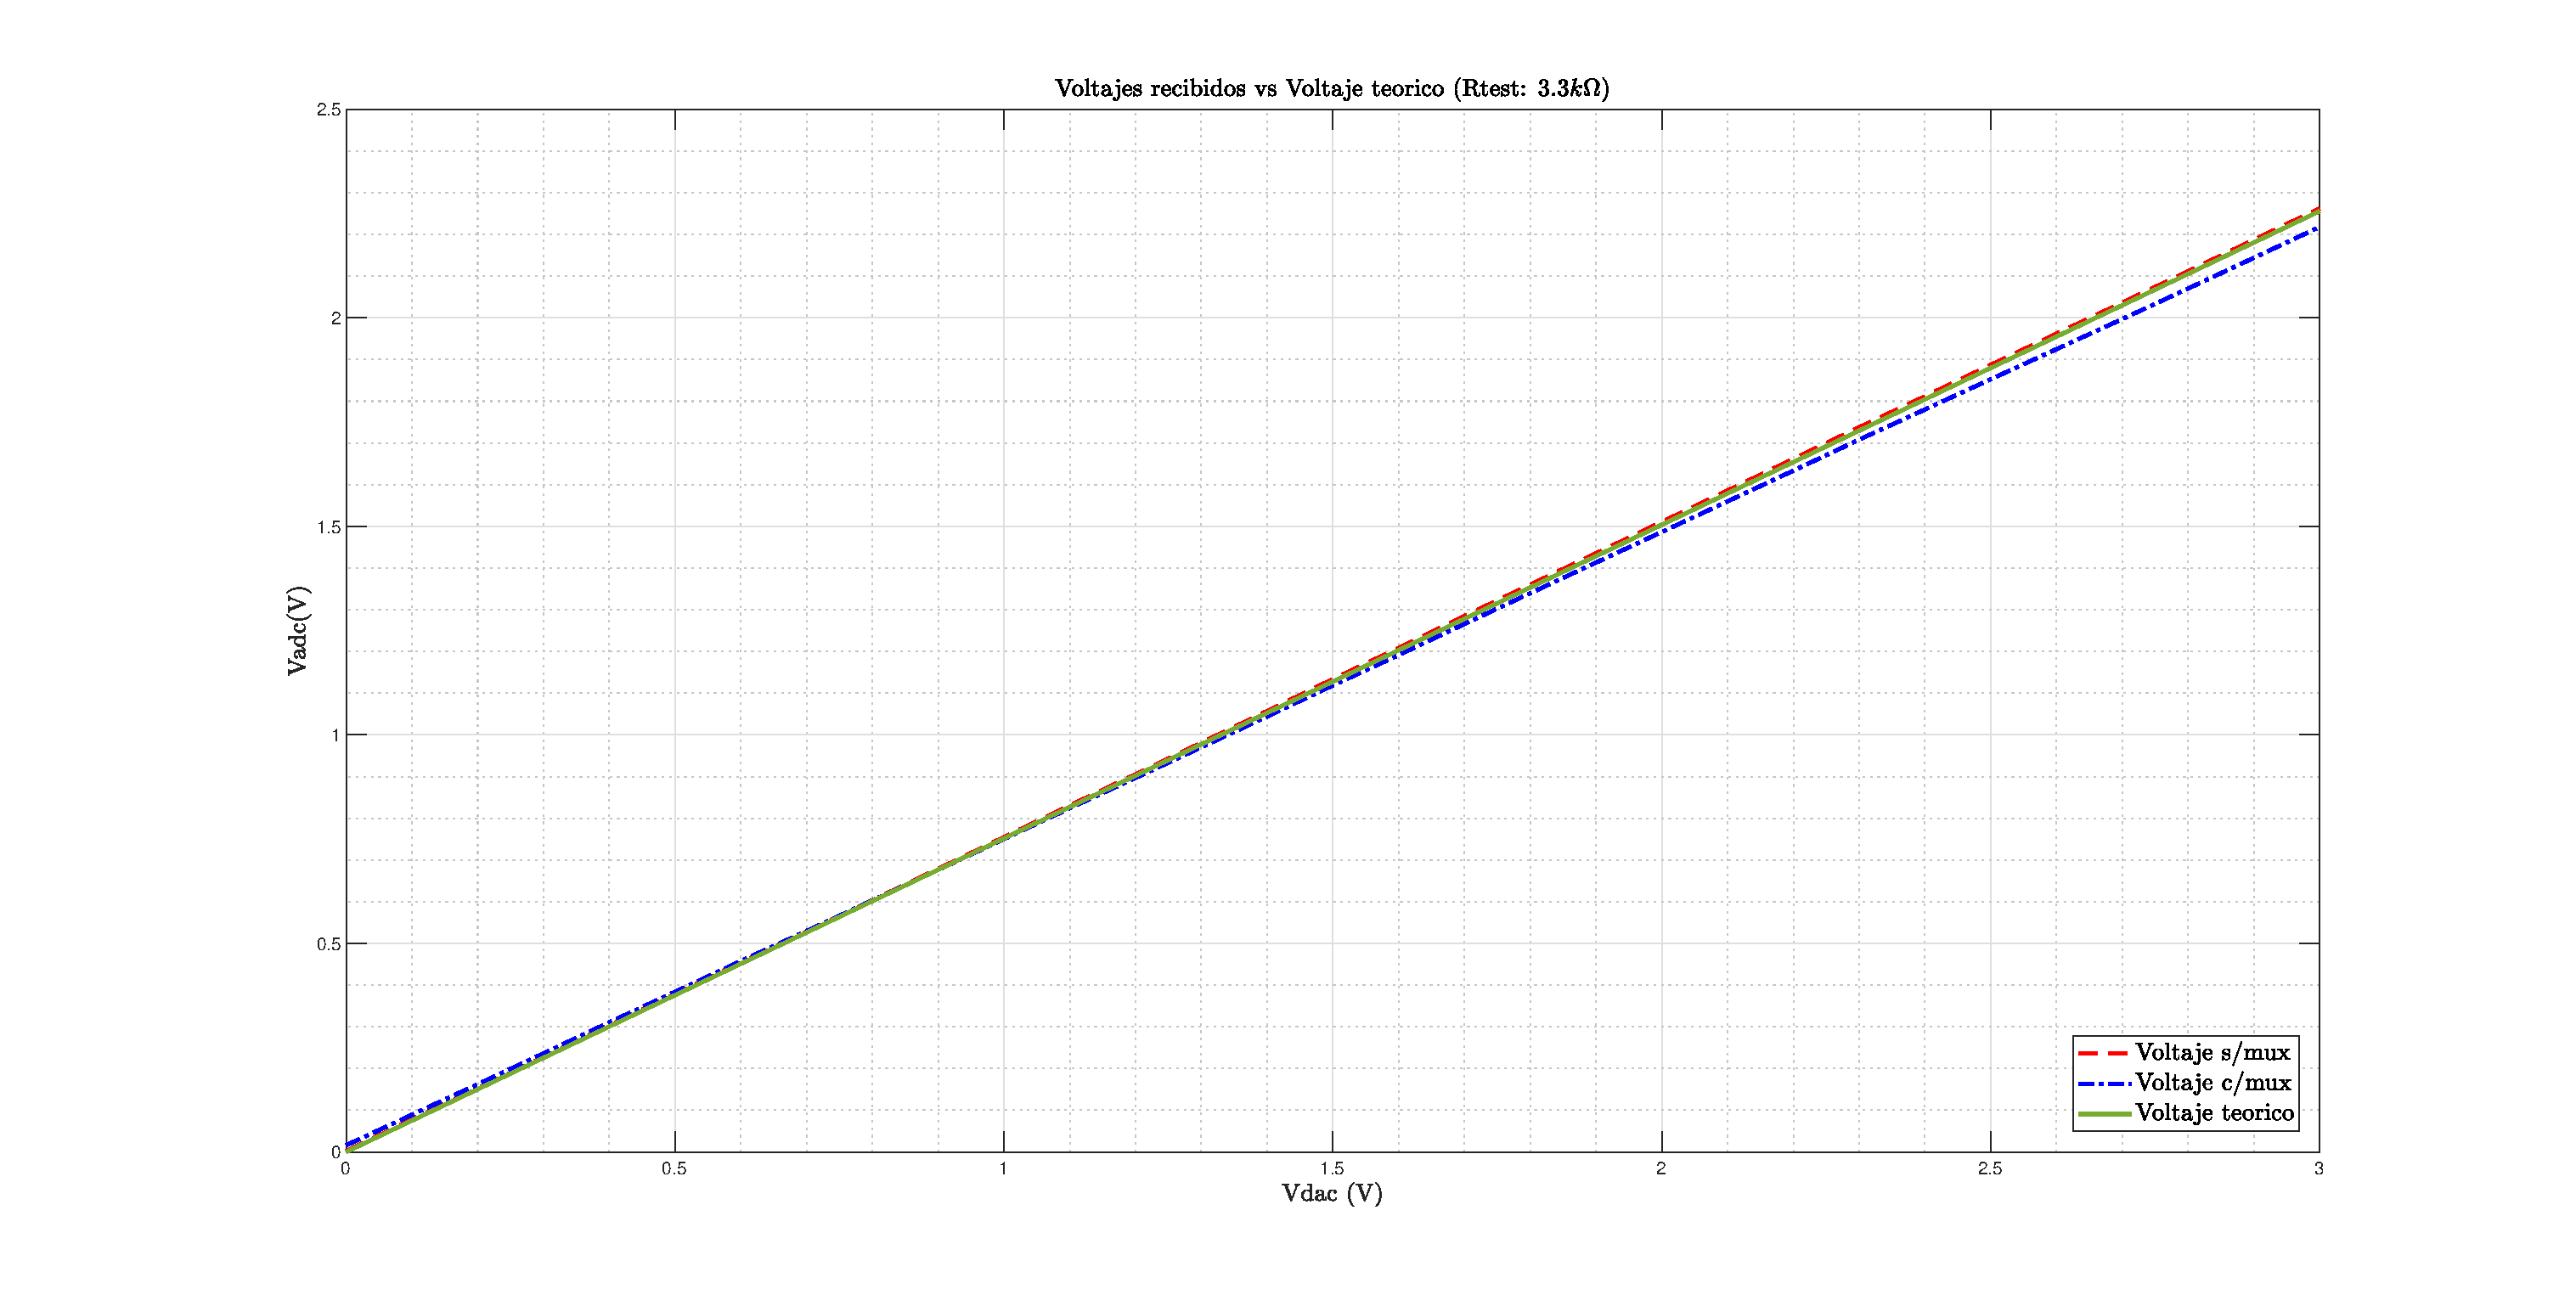
\includegraphics[width=1\textwidth]{02_3k3_new}
                \caption{Influencia de resistencia de multiplexores.}
                \label{fig:02_3k3_new}
            \end{figure}              
 
            \begin{figure}[hbtp]
                \centering
                \includegraphics[width=1\textwidth]{03_5k6_new}
                \caption{Influencia de resistencia de multiplexores.}
                \label{fig:03_5k6_new}
            \end{figure}   

            \begin{figure}[hbtp]
                \centering
                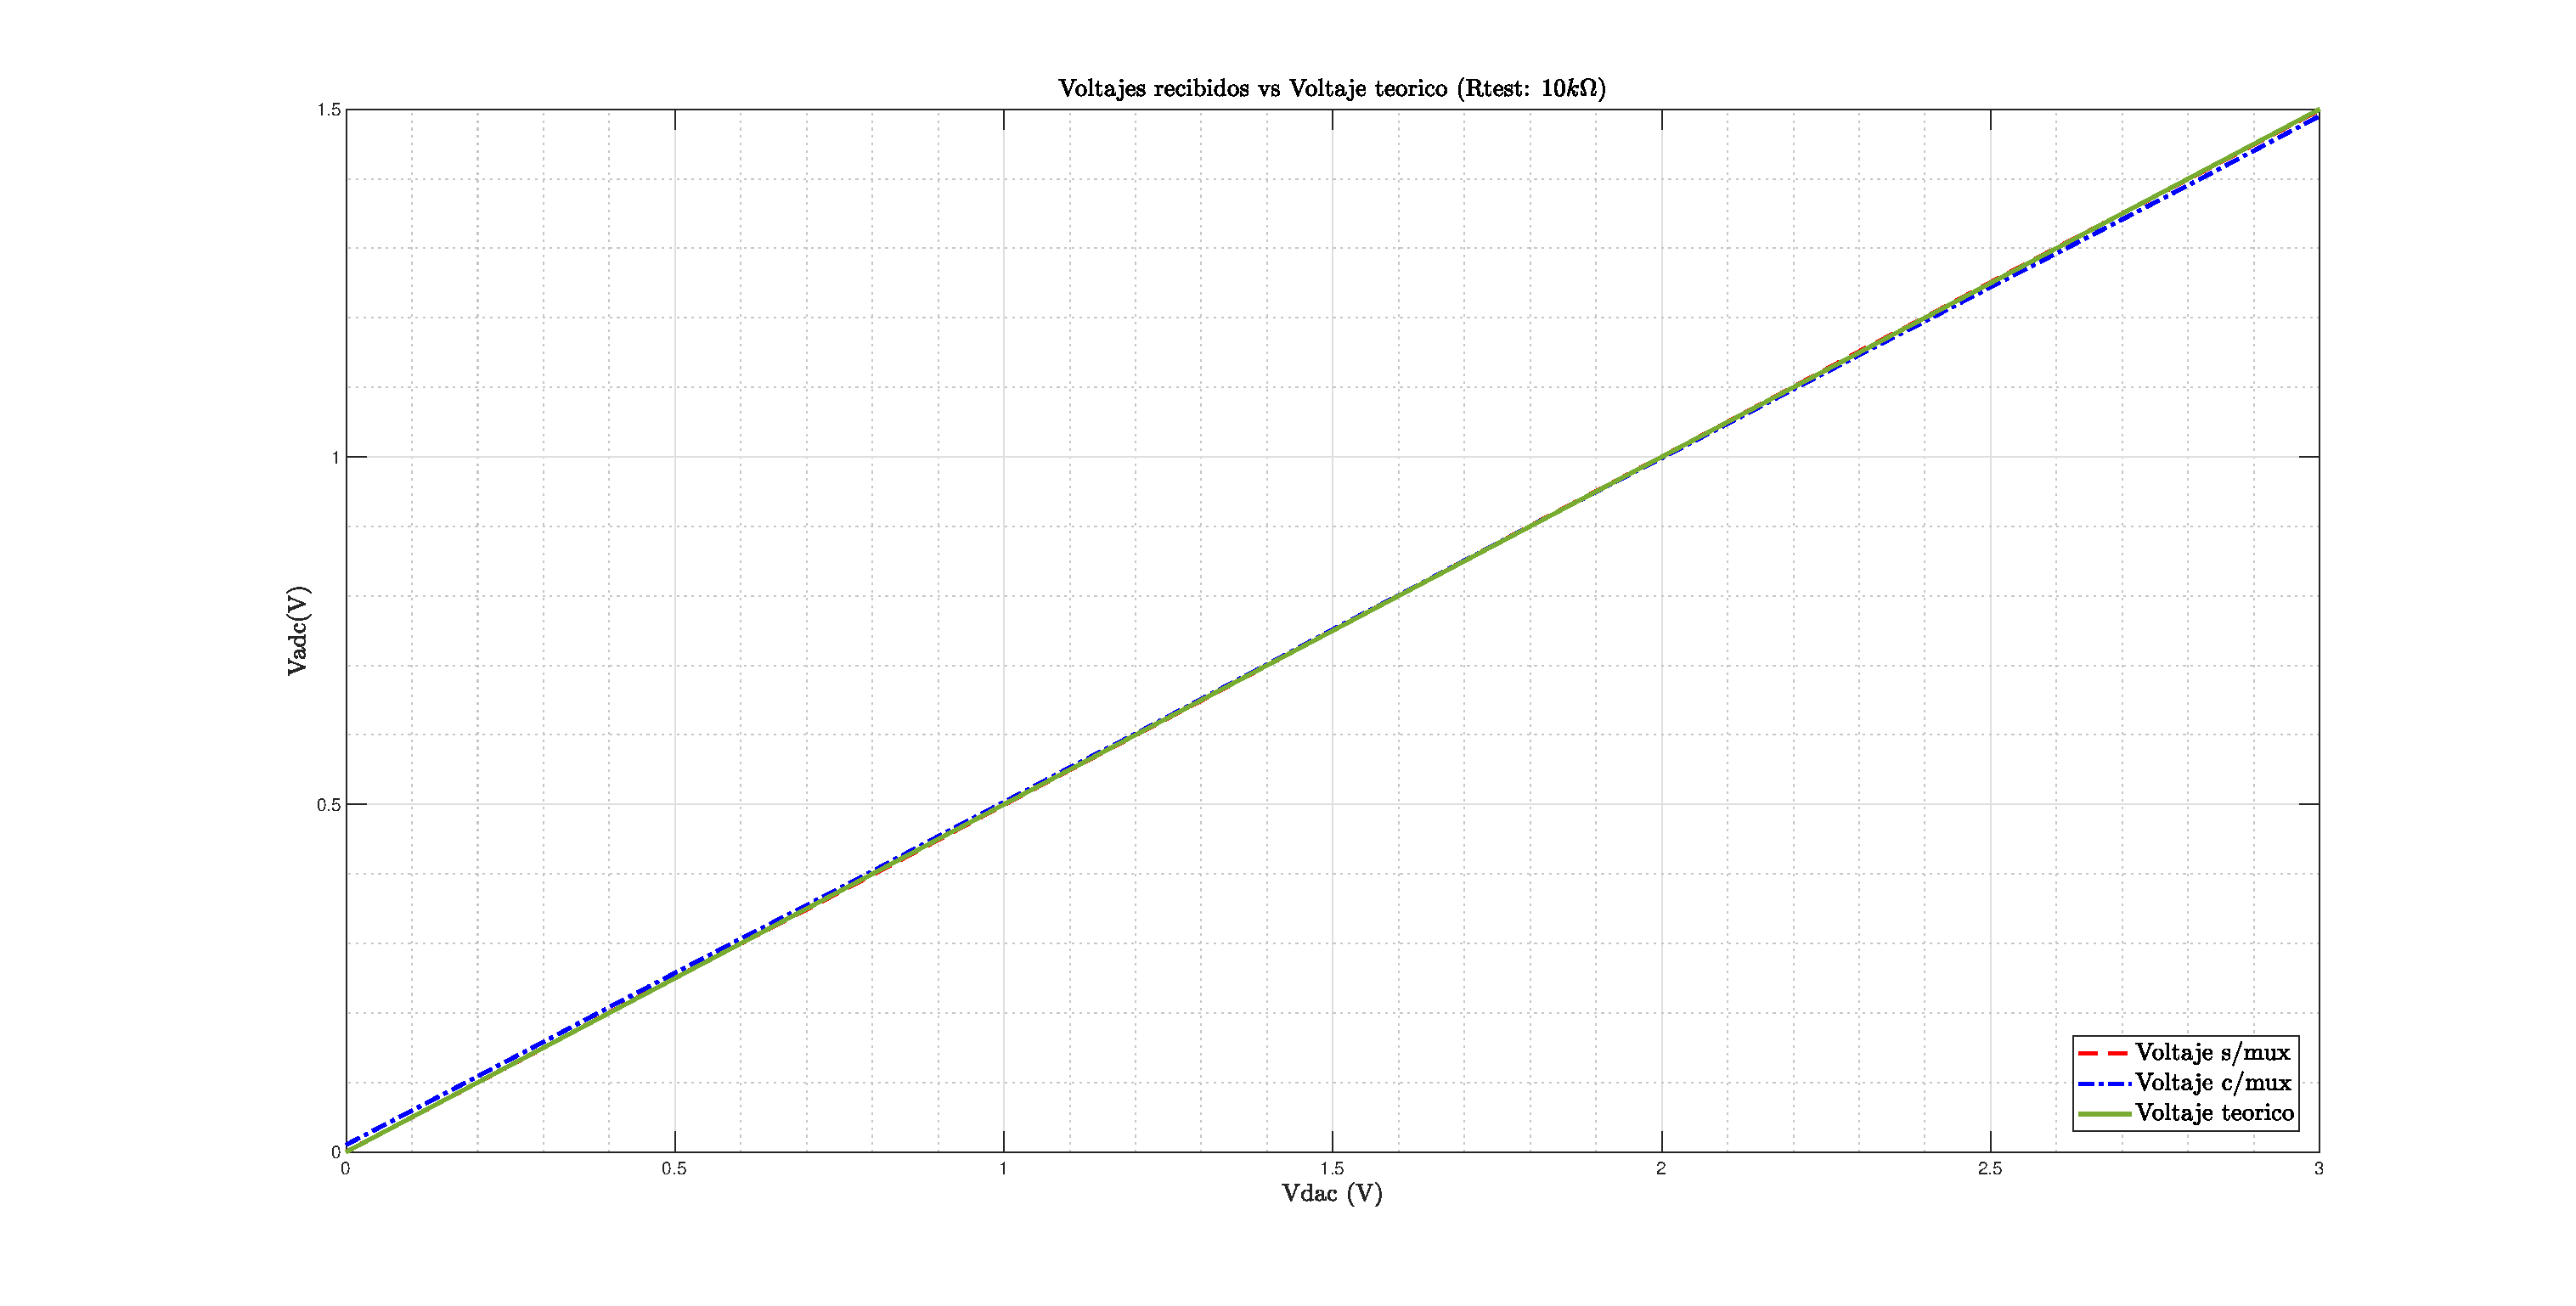
\includegraphics[width=1\textwidth]{04_10k_new}
                \caption{Influencia de resistencia de multiplexores.}
                \label{fig:04_10k_new}
            \end{figure}  
                
                     
\section{Resultados de caracterización de fotorresistencias}

            \begin{table}[htbp]
                \caption{Valor de fotorresistencias con diferentes duty cycles.}
                \begin{center}
                    \resizebox{0.6\linewidth}{!}{ 
                    \begin{NiceTabular}{| c | c | c |}
                        \CodeBefore
                        \Body
                        \hline
                        \textbf{$V_{Fuente}$}  & \textbf{Duty cycle ($\%$)} & \textbf{$R_{med} (K\Omega)$} \\
                        \hline
                        3 V     & 25  & 210 - 213.7\\
                                & 50  & 104 - 105.7\\
                                & 75  & 70 -71\\
                                & 100 & 53 - 54\\ \hline
                        3.3 V   & 25  & 29 - 31\\
                                & 50  & 16 - 17\\
                                & 75  & 11 - 12\\
                                & 100 & 8 - 9\\ \hline
                        3.5 V   & 25  & 6 - 7\\
                                & 50  & 3.6\\
                                & 75  & 2.6\\
                                & 100 & 2\\                             
                        \hline
                    \end{NiceTabular}
                    }
                \label{tab:Duty_cycle}
                \end{center}
            \end{table}


            \begin{figure}[hbtp]
                \centering
                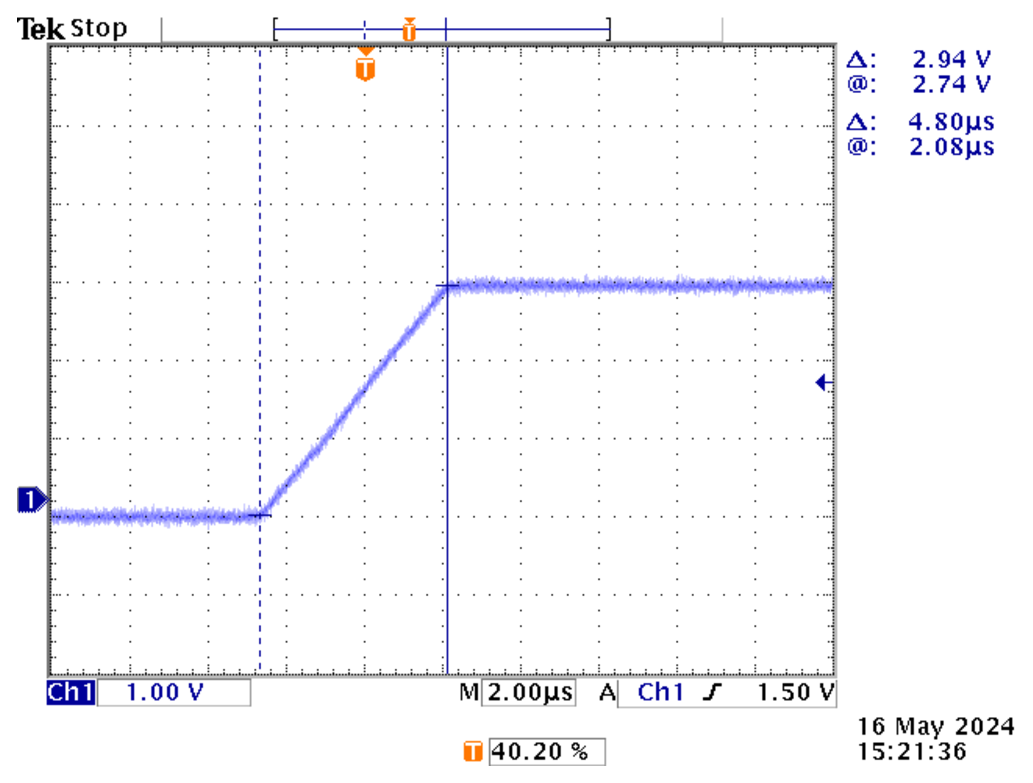
\includegraphics[width=0.6\textwidth]{settling_3v}
                \caption{Captura de osciloscopio de settling time.}
                \label{fig:settling_3v}
            \end{figure}
            
            \begin{figure}[hbtp]
                \centering
                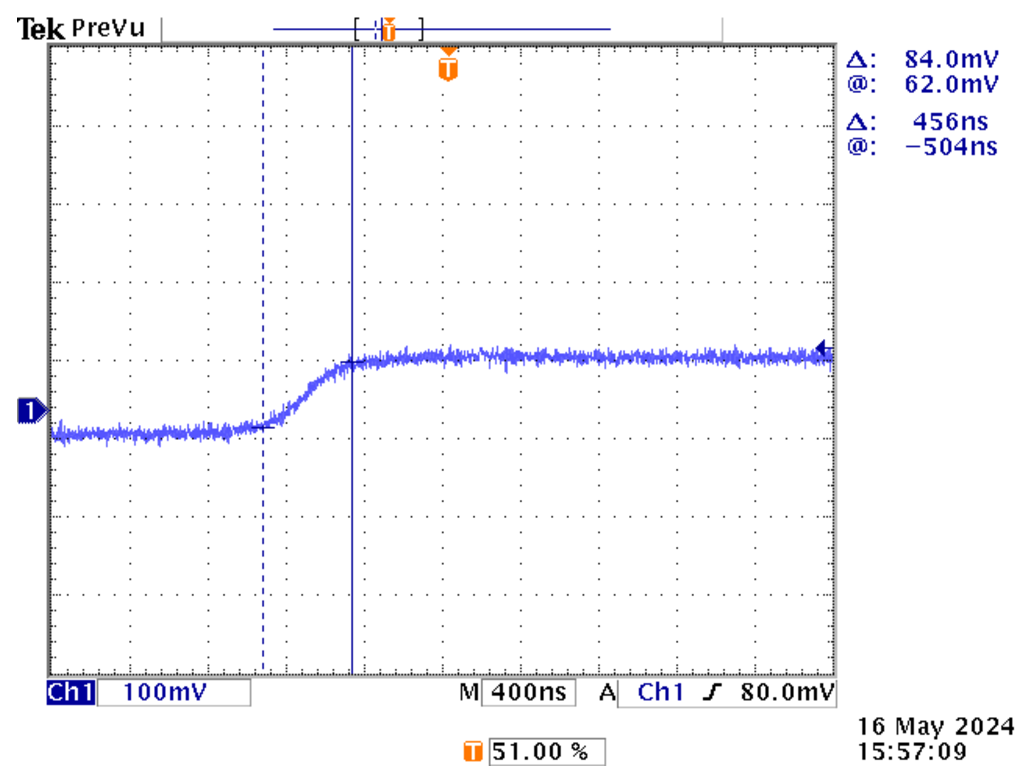
\includegraphics[width=0.6\textwidth]{settling_0v1}
                \caption{Captura de osciloscopio de settling time.}
                \label{fig:settling_0v1}
            \end{figure} 
            
            \begin{figure}[hbtp]
                \centering
                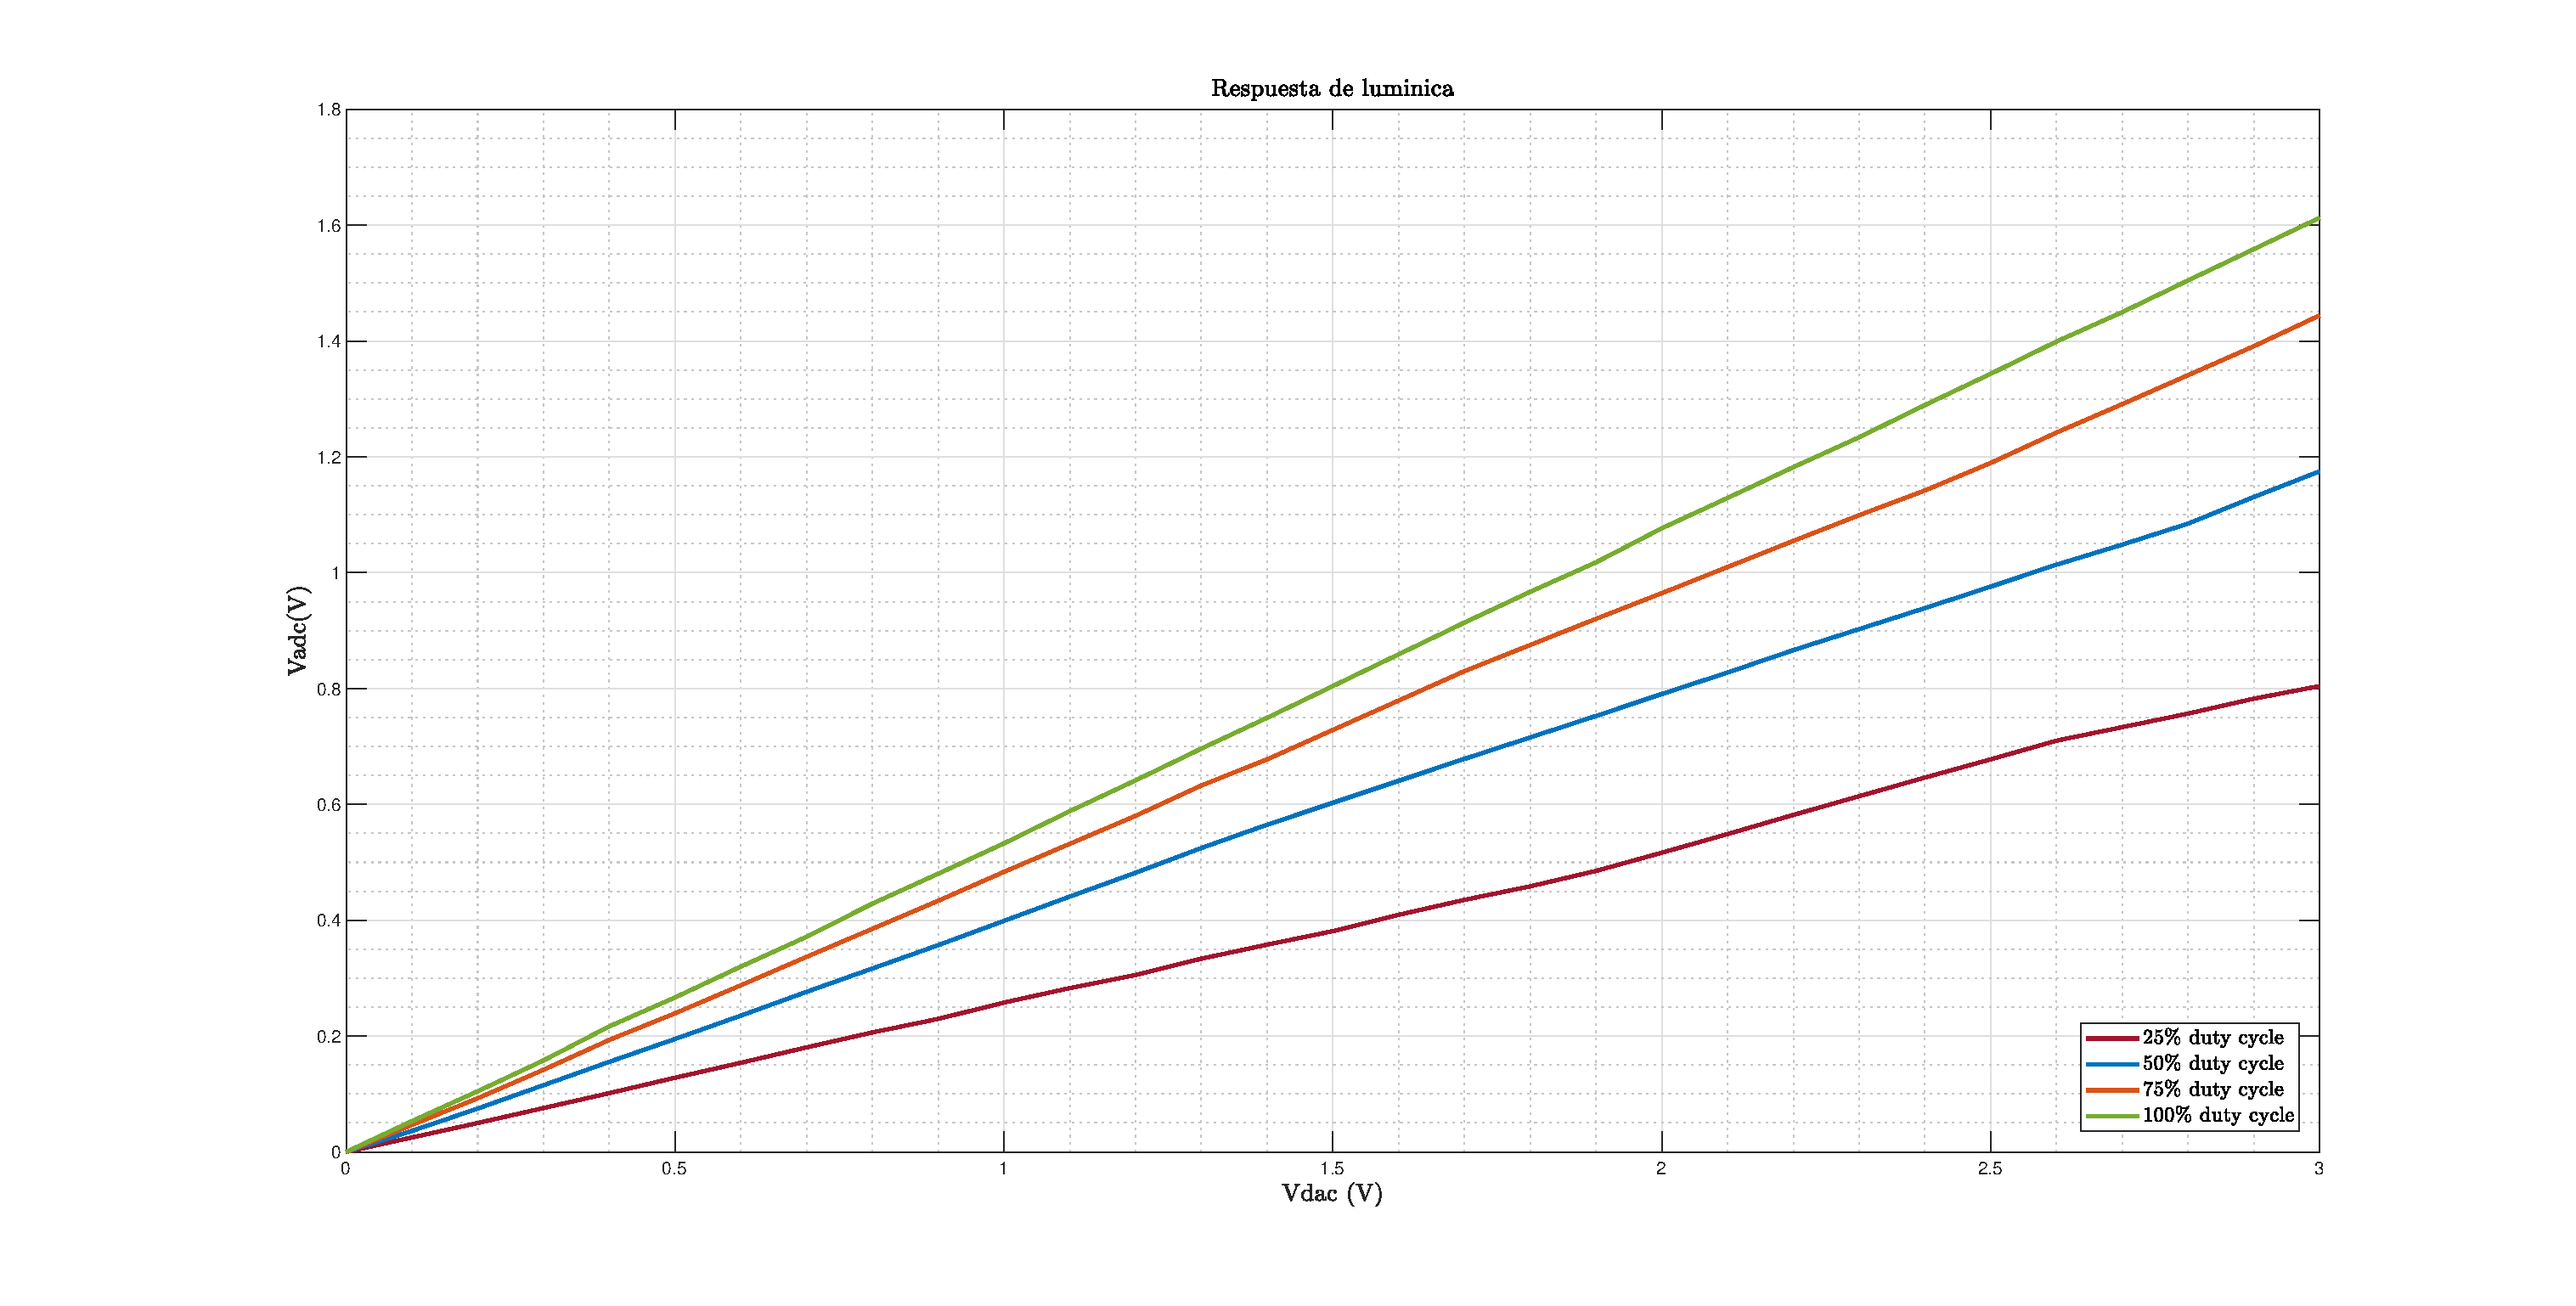
\includegraphics[width=1\textwidth]{respuesta_luminica}
                \caption{Respuesta lumínica.}
                \label{fig:respuesta_luminica}
            \end{figure}            
            
            

\section{Imágenes obtenidas}

            \begin{figure}[hbtp]
                \centering
                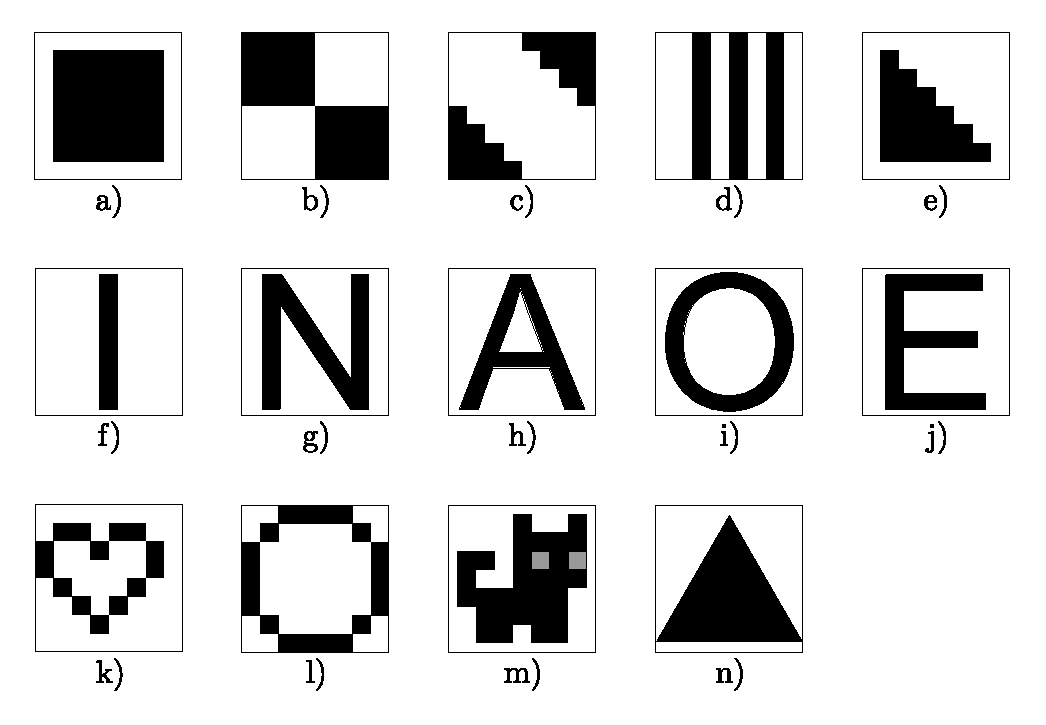
\includegraphics[width=0.8\textwidth]{mask_final}
                \caption{Máscaras aplicadas a matriz de fototransistores.}
                \label{fig:mask_final}
            \end{figure}  

            \begin{figure}[hbtp]
                \centering
                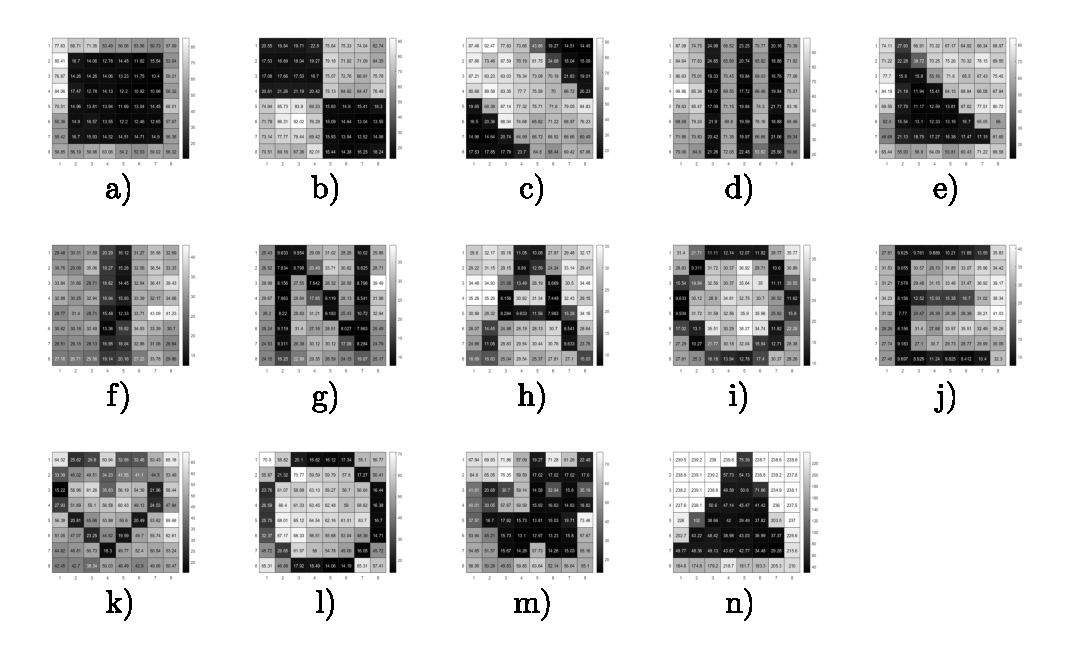
\includegraphics[width=0.8\textwidth]{result_mask}
                \caption{Resultados de las máscaras aplicadas a los fototransistores.}
                \label{fig:result_mask}
            \end{figure}
